\documentclass{article}

\usepackage{graphicx}
\usepackage{tikz}
\usepackage{tikzsymbols}
\usetikzlibrary{calc,patterns,shapes.geometric}
\pagestyle{empty}
\usepackage[margin=0pt]{geometry}
\geometry{papersize={14in,12in}}

\def\centerarc[#1](#2)(#3:#4:#5){\draw[#1] ($(#2)+({#5*cos(#3)},{#5*sin(#3)})$) arc (#3:#4:#5);}

\begin{document}
	\begin{figure}
		\centering
		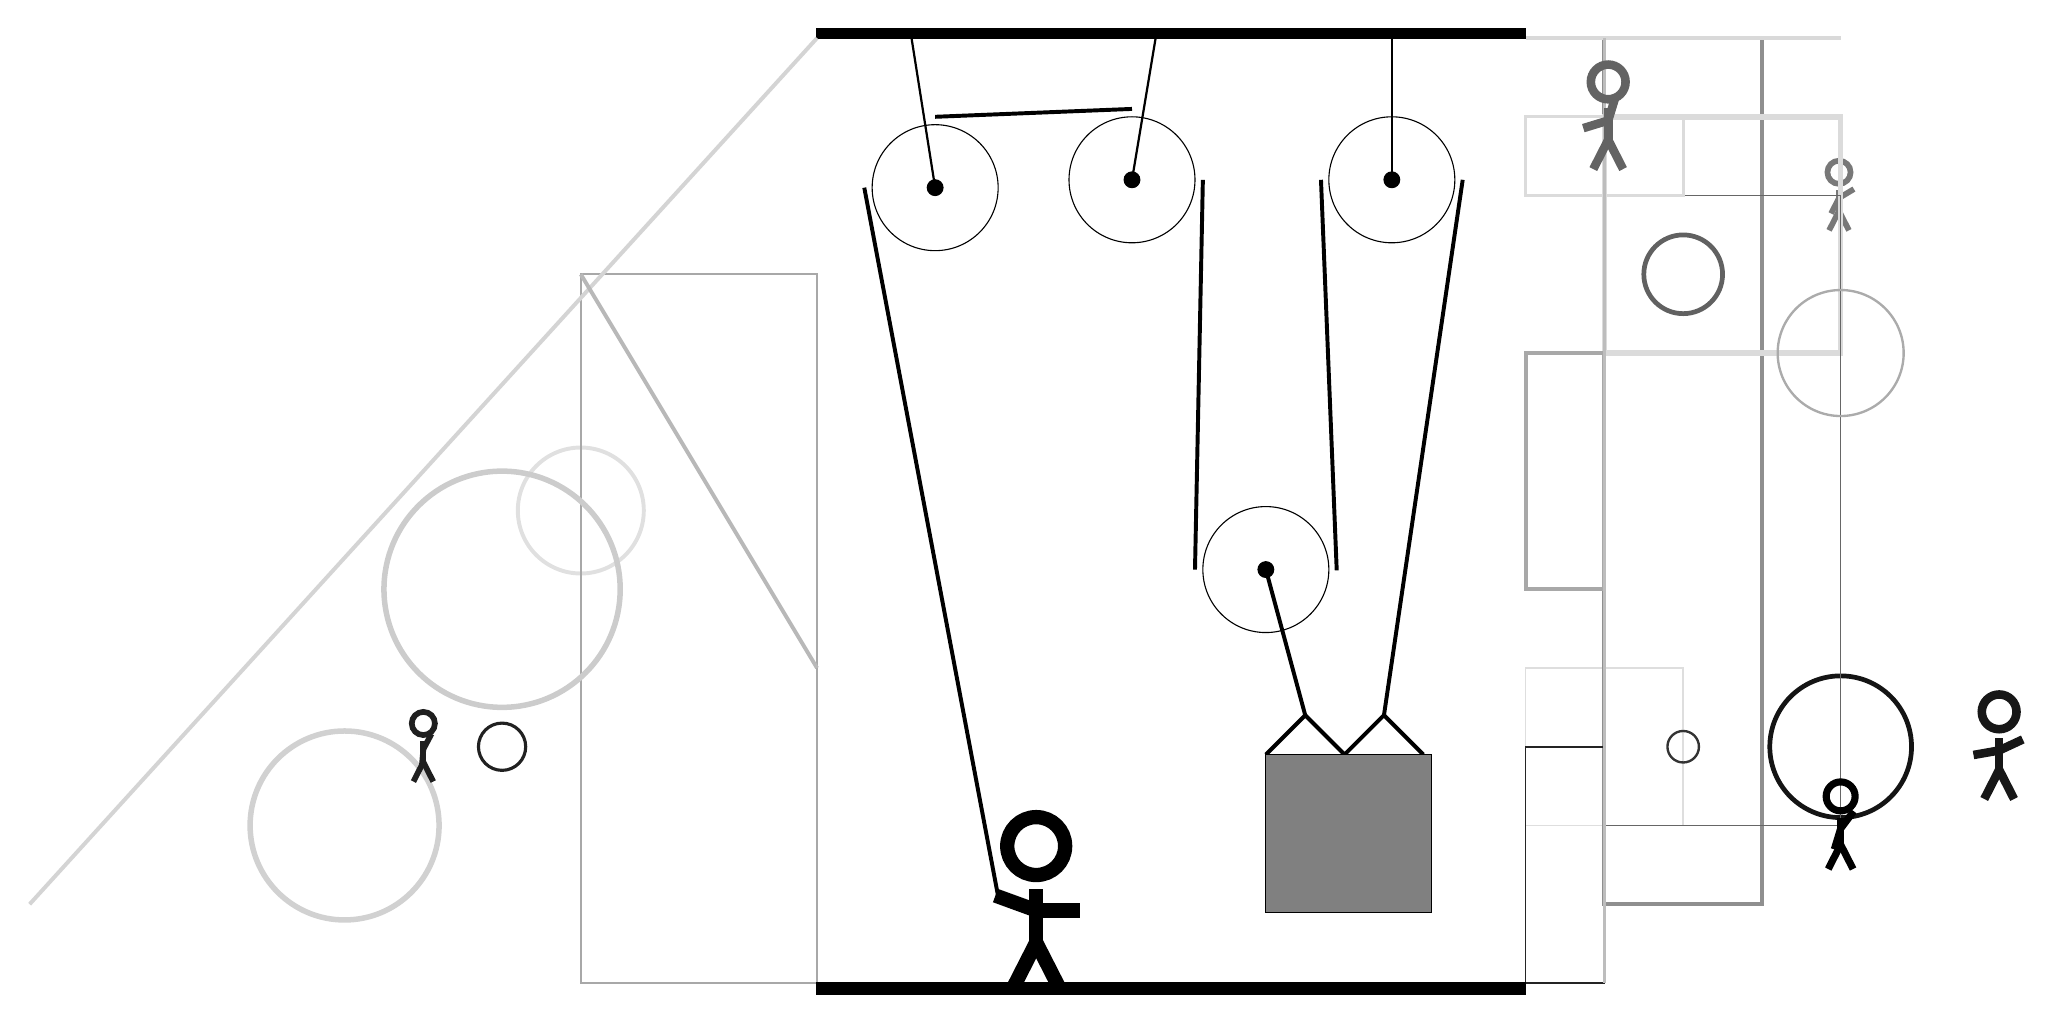
\begin{tikzpicture}
			%%%%% START %%%%%
			
			\draw[fill=black] (-3, 9) rectangle (6, 9.125);
			
			\draw (1, 7.2) circle (0.8);
			\draw[fill=black] (1, 7.2) circle (0.1);
			\draw[thick] (1, 7.2) -- (1.3, 9);
			
			\draw (4.3, 7.2) circle (0.8);
			\draw[fill=black] (4.3, 7.2) circle (0.1);
			\draw[thick] (4.3, 7.2) -- (4.3, 9);
			
			\draw (2.7, 2.25) circle (0.8);
			\draw[fill=black] (2.7, 2.25) circle (0.1);
			
			\draw[line width=0.5mm]  (2.7, -0.1) -- (3.2, 0.4) -- (3.7, -0.1) -- (4.2, 0.4) -- (4.7, -0.1);
			\draw[fill=black!50] (2.7, -0.1) rectangle (4.8, -2.1);
			
			\draw (-1.5, 7.1) circle (0.8);
			\draw[fill=black] (-1.5, 7.1) circle (0.1);
			\draw[thick] (-1.5, 7.1) -- (-1.8, 9);
			
			\draw[line width=0.5mm](-0.7, -1.9) --  (-2.4, 7.1);
			\centerarc[line width=0.5mm](-1.5, 7.1)(90:180:0.9);
			\draw[line width=0.5mm](-1.5, 8.0) -- (1, 8.1);
			\centerarc[line width=0.5mm](1, 7.2)(0:90:0.9);
			\draw[line width=0.5mm](1.9, 7.2) -- (1.8, 2.25);
			\centerarc[line width=0.5mm](2.7, 2.25)(180:370:0.9);
			\draw[line width=0.5mm] (3.6, 2.24) -- (3.4, 7.2);
			\centerarc[line width=0.5mm](4.3, 7.2)(0:180:0.9);
			\draw[line width=0.5mm](4.2, 0.4) -- (5.2, 7.2);
			\draw[line width=0.5mm] (3.2, 0.4) -- (2.7, 2.25);
			
			\draw [line width=0.6mm, color=black!92](10, 0) circle (0.9);
			
			\draw[line width=0.2mm, color=black!13] (8, -1) rectangle (6, 1);
			\draw[line width=0.5mm, color=black!44] (7, -2) rectangle (9, 9);
			\draw [line width=0.5mm, color=black!12](-6, 3) circle (0.8);
			\draw[line width=0.2mm, color=black!34] (-3, -3) rectangle (-6, 6);
			
			\draw [line width=0.7mm, color=black!20](-7, 2) circle (1.5);
			\draw [line width=0.7mm, color=black!18](-9, -1) circle (1.2);
			\node[line width=0.2mm, color=black!53] at (10, 7) {\Strichmaxerl[4][63][31]};
			\draw[line width=0.5mm, color=black!17](-3, 9) -- (-13, -2);
			\draw[line width=0.7mm, color=black!14] (7, 8) rectangle (10, 5);
			\draw[line width=0.2mm, color=black!86] (6, 0) rectangle (7, -3);
			\draw[line width=0.2mm, color=black!60] (7, -1) rectangle (10, 7);
			\draw[line width=0.5mm, color=black!28](-6, 6) -- (-3, 1);
			\node[line width=0.2mm, color=black!100] at (10, -1) {\Strichmaxerl[5][73][53]};
			\node[line width=0.2mm, color=black!88] at (-8, 0) {\Strichmaxerl[4][85][62]};
			\draw[line width=0.4mm, color=black!14] (8, 8) rectangle (6, 7);
			
			\draw[line width=0.5mm, color=black!15](10, 9) -- (6, 9);
			
			\draw [line width=0.6mm, color=black!62](8, 6) circle (0.5);
			\draw[line width=0.5mm, color=black!34] (7, 5) rectangle (6, 2);
			\draw [line width=0.3mm, color=black!33](10, 5) circle (0.8);
			\draw[line width=0.3mm, color=black!26] (7, -3) rectangle (7, 9);
			\draw [line width=0.4mm, color=black!87](-7, 0) circle (0.3);
			\draw [line width=0.3mm, color=black!80](8, 0) circle (0.2);
			\node[line width=0.3mm, color=black!61] at (7, 8) {\Strichmaxerl[6][17][73]};
			\node[line width=0.5mm, color=black!91] at (12, 0) {\Strichmaxerl[6][10][25]};
			
			
			\node at (-0.2, -2) {\Strichmaxerl[10][-20][0]};
			
			\draw[fill=black] (-3, -3) rectangle (6, -3.15);
			
			%%%%% END %%%%%
		\end{tikzpicture}
	\end{figure}	
\end{document}